\begin{section}{N-body Simulation of Dark Matter Density Fields}
  \label{sec:simulation}
    We run 136 simulations with a box size of 300 $h^{-1}$Mpc, 
resolution of $1024^3$ cells and $512^3$ particles, using the cosmological 
simulation code CubeP3M\cite{bib:Harnois2013}. The initial condition is 
given by reading the transfer function computed by CAMB \cite{bib:Lewis2000} 
and then evolving the power linearly to $z=100$. Then Zel'dovich approximation 
is used to calculate the displacement field and velocity field, which are 
assigned to the particles. The cosmological parameters used are $\Omega_M=0.32$, 
$\Omega_{\Lambda}=0.679$, $h=0.67$, $\sigma_8=0.83$, and $n_s=0.96$.Then the 
initial densities are evolved up to $z=0$. Different seeds are used to produce 
the initial conditions for different simulations so that those simulations are 
indipendent to each other.
\begin{figure*}[t!]
\centering
 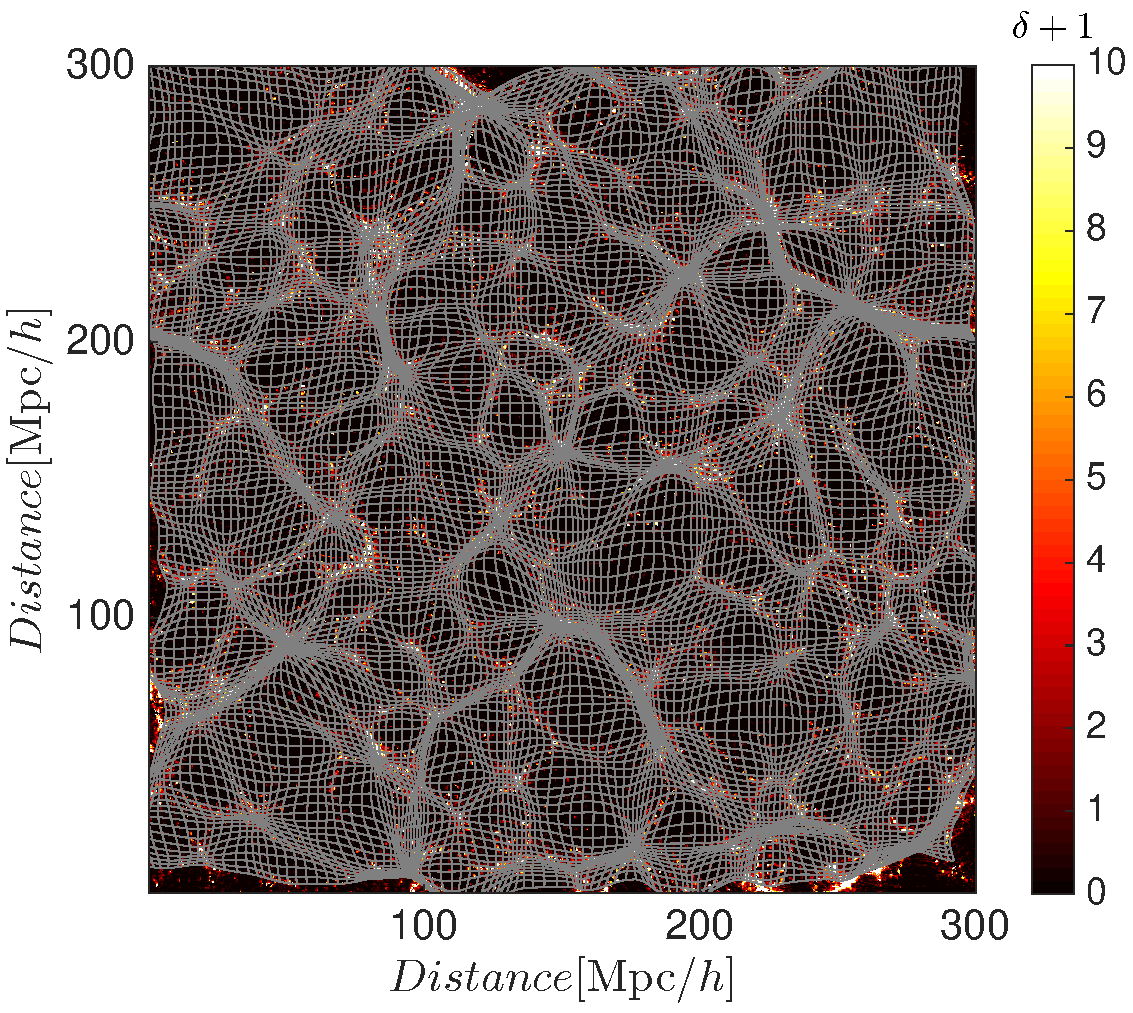
\includegraphics[width=0.9\textwidth]{sar_best_analysis-crop.pdf}
 \label{fig:simandrec}
   \caption{
2-D projection of one
layer of the deformed grids of one out of 136 N-body simulations, and the density field 
on the selected deformed grids, with the magnitude as the number of particles per cell. 
The simulations hace 300 $h^{-1}$Mpc width box and $1024^3$ pixels.}
\end{figure*}

\end{section}

